\section{CLocation\-Event$<$ T $>$::CGeneric\-Location\-Reactor$<$ U $>$  Class Template Reference}
\label{classCLocationEvent_1_1CGenericLocationReactor}\index{CLocationEvent::CGenericLocationReactor@{CLocation\-Event::CGeneric\-Location\-Reactor}}
Inheritance diagram for CLocation\-Event$<$ T $>$::CGeneric\-Location\-Reactor$<$ U $>$::\begin{figure}[H]
\begin{center}
\leavevmode
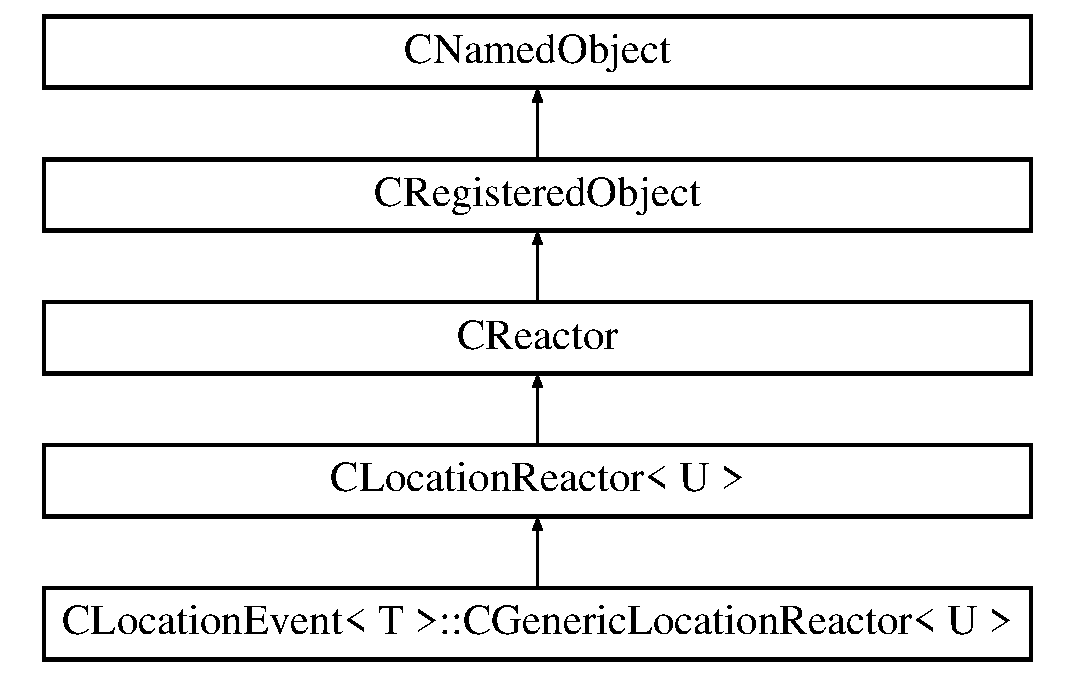
\includegraphics[height=5cm]{classCLocationEvent_1_1CGenericLocationReactor}
\end{center}
\end{figure}
\subsection*{Public Methods}
\begin{CompactItemize}
\item 
{\bf CGeneric\-Location\-Reactor} ({\bf CLocation\-Event}$<$ T $>$ \&r\-Owner)
\item 
virtual void {\bf On\-Location\-Changed} ({\bf CLocation\-Monitor}$<$ T $>$ \&r\-Event, T New\-Value)
\item 
virtual void {\bf On\-Timeout} ({\bf CEvent\-Monitor} \&r\-Event)
\end{CompactItemize}
\subsection*{Private Attributes}
\begin{CompactItemize}
\item 
{\bf CLocation\-Event}$<$ T $>$ \& {\bf m\_\-r\-Owner}
\end{CompactItemize}


\subsection{Detailed Description}
\subsubsection*{template$<$class T$>$template$<$class U$>$ class CLocation\-Event$<$ T $>$::CGeneric\-Location\-Reactor$<$ U $>$}

Nested class CLocation\-Event::CLocation\-Reactor This class is used to give events a monolithic appearance. They relay calls to the Reactor action member functions to corresponding event members. This allows the user of this class to create response by simply subclassing this class rather than forcing them to be aware of the relationship between monitors and reactors. 



Definition at line 348 of file CLocation\-Event.h.

\subsection{Constructor \& Destructor Documentation}
\index{CLocationEvent::CGenericLocationReactor@{CLocation\-Event::CGeneric\-Location\-Reactor}!CGenericLocationReactor@{CGenericLocationReactor}}
\index{CGenericLocationReactor@{CGenericLocationReactor}!CLocationEvent::CGenericLocationReactor@{CLocation\-Event::CGeneric\-Location\-Reactor}}
\subsubsection{\setlength{\rightskip}{0pt plus 5cm}template$<$class T$>$ template$<$class U$>$ {\bf CLocation\-Event}$<$ T $>$::CGeneric\-Location\-Reactor$<$ U $>$::CGeneric\-Location\-Reactor ({\bf CLocation\-Event}$<$ T $>$ \& {\em r\-Owner})}\label{classCLocationEvent_1_1CGenericLocationReactor_a0}


Constructor. Builds a location reactor for {\bf CLocation\-Event} {\rm (p.\,\pageref{classCLocationEvent})} objects. We just keep track of our 'owner' so we know how to callback.\begin{Desc}
\item[Parameters: ]\par
\begin{description}
\item[{\em 
r\-Owner}]- Reference to our owner object. \end{description}
\end{Desc}


Definition at line 308 of file CLocation\-Event.cpp.

\subsection{Member Function Documentation}
\index{CLocationEvent::CGenericLocationReactor@{CLocation\-Event::CGeneric\-Location\-Reactor}!OnLocationChanged@{OnLocationChanged}}
\index{OnLocationChanged@{OnLocationChanged}!CLocationEvent::CGenericLocationReactor@{CLocation\-Event::CGeneric\-Location\-Reactor}}
\subsubsection{\setlength{\rightskip}{0pt plus 5cm}template$<$class T$>$ template$<$class U$>$ void {\bf CLocation\-Event}$<$ T $>$::CGeneric\-Location\-Reactor$<$ U $>$::On\-Location\-Changed ({\bf CLocation\-Monitor}$<$ T $>$ \& {\em r\-Event}, T {\em New\-Value})\hspace{0.3cm}{\tt  [virtual]}}\label{classCLocationEvent_1_1CGenericLocationReactor_a1}


Called when the location has changed in a manner which is significant to the predicate attached to the event. We delegate the action to the Event object which owns us presenting a monolithic appearance of events to the experimenter.\begin{Desc}
\item[Parameters: ]\par
\begin{description}
\item[{\em 
r\-Event}]- Event which fired the operation. \item[{\em 
New\-Value}]- New value in the location. \end{description}
\end{Desc}


Definition at line 326 of file CLocation\-Event.cpp.

References CLocation\-Event$<$ T $>$::CGeneric\-Location\-Reactor$<$ U $>$::m\_\-r\-Owner.\index{CLocationEvent::CGenericLocationReactor@{CLocation\-Event::CGeneric\-Location\-Reactor}!OnTimeout@{OnTimeout}}
\index{OnTimeout@{OnTimeout}!CLocationEvent::CGenericLocationReactor@{CLocation\-Event::CGeneric\-Location\-Reactor}}
\subsubsection{\setlength{\rightskip}{0pt plus 5cm}template$<$class T$>$ template$<$class U$>$ void {\bf CLocation\-Event}$<$ T $>$::CGeneric\-Location\-Reactor$<$ U $>$::On\-Timeout ({\bf CEvent\-Monitor} \& {\em r\-Event})\hspace{0.3cm}{\tt  [virtual]}}\label{classCLocationEvent_1_1CGenericLocationReactor_a2}


Called when timeout receipt is enabled, and a wait times out.  This function delegates action tot he event object which owns us, presenting a monolithic appearance of events to the experimentalist.\begin{Desc}
\item[Parameters: ]\par
\begin{description}
\item[{\em 
r\-Event}]- Reference to the monitor which timed out. (unused). \end{description}
\end{Desc}


Reimplemented from {\bf CReactor} {\rm (p.\,\pageref{classCReactor_a8})}.

Definition at line 342 of file CLocation\-Event.cpp.

References CLocation\-Event$<$ T $>$::CGeneric\-Location\-Reactor$<$ U $>$::m\_\-r\-Owner.

\subsection{Member Data Documentation}
\index{CLocationEvent::CGenericLocationReactor@{CLocation\-Event::CGeneric\-Location\-Reactor}!m_rOwner@{m\_\-rOwner}}
\index{m_rOwner@{m\_\-rOwner}!CLocationEvent::CGenericLocationReactor@{CLocation\-Event::CGeneric\-Location\-Reactor}}
\subsubsection{\setlength{\rightskip}{0pt plus 5cm}template$<$class T$>$ template$<$class U$>$ {\bf CLocation\-Event}$<$T$>$\& {\bf CLocation\-Event}$<$ T $>$::CGeneric\-Location\-Reactor$<$ U $>$::m\_\-r\-Owner\hspace{0.3cm}{\tt  [private]}}\label{classCLocationEvent_1_1CGenericLocationReactor_o0}




Definition at line 351 of file CLocation\-Event.h.

Referenced by CLocation\-Event$<$ T $>$::CGeneric\-Location\-Reactor$<$ U $>$::On\-Location\-Changed(), and CLocation\-Event$<$ T $>$::CGeneric\-Location\-Reactor$<$ U $>$::On\-Timeout().

The documentation for this class was generated from the following files:\begin{CompactItemize}
\item 
{\bf CLocation\-Event.h}\item 
{\bf CLocation\-Event.cpp}\end{CompactItemize}
